\graphicspath{{sections/MARVINWOLF/images/}}

\section[Überblick]{Überblick \myAuthor{Marvin Wolf}}

\subsection{Architekturübersicht}

\begin{figure}[ht]
    \centering
    
\includegraphics[width=1\textwidth]{Architecture.png}
    \caption{Architekturübersicht grob}
\end{figure}

Das Team Digitalize macht Aufnahmen der Puzzleteile. Diese werden von der Rohform (RAW-Format) in ein nutzbares Format gewandelt. Auf diesem wird dann die Segmentierung des Puzzleteils vom Hintergrund vorgenommen, d.h. das Teil wird ausgeschnitten. Zusätzlich wird es einheitlich skaliert, so dass die Puzzleteile ihrem Originalmaß entsprechen. Zuletzt wird das segmentierte Puzzleteil auf einen transparenten Hintergrund gelegt sowie ein SVG-File erzeugt, dass den Rand beschreibt. Diese Resultate werden von den Solvern für das Lösen des Puzzles genutzt sowie von den Visualizern für das Anzeigen der Puzzleteile.
\newline Die Gruppe Solve extrahiert im Preprocessing wichtige Merkmale für das Lösen des Puzzles. Dabei werden die Kanten jedes Puzzleteiles mit jeder Kante aller anderen Puzzleteile verglichen und ein Wahrschneinlichkeitsmaß für deren Zusammenpassen gebildet. Die Methoden Edge Matching und XOR Matching vergleicht die Kantenform der Puzzleteile. Das Farbmatching vergleicht den Farbverlauf zweier Kanten.
Die entstehenden Wahrscheinlichkeitsmatrizen dienen dem Solver Algorithmus als Eingabe, um das Puzzle zu lösen. Er gibt das gelöste Puzzle in Form einer 7x7 Matrix aus. Das Post-Processing wird benötigt, um die Rotation und Position der Puzzleteile zu berechnen, so dass die Teile ineinander passen und das Puzzle eine lückenlos gefüllte Fläche ergibt. 
\newline Diese Informationen nutzt das Team Control, um die Bewegung des Roboterarms von einer fest definierten Startposition zu der jeweiligen Endposition zu berechnen. Diese Bewegung wird in Form einer Abfolge von Winkeln, die die Arme des Roboters zueinander haben und so dessen Anordnung beschreiben, an Visualize weitergegeben.
\newline Die Gruppe Visualize liefert ein Graphical User Interface, in dem der Roboter und das Lösen des Puzzles animiert werden. Die Puzzleteile liegen auf einem Stapel und werden nach und nach vom Roboter gegriffen und an die korrekte Stelle gesetzt. Die Drehung des Puzzleteiles ist bereits zur Initlalisierung gegeben d.h. das Teil muss nur bewegt werden. Die Aufgabe ist gelöst, sobald alle Puzzleteile ausgebreitet sind und ein komplett zusammengesetztes Puzzle ergeben.

\begin{figure}[ht]
    \centering
    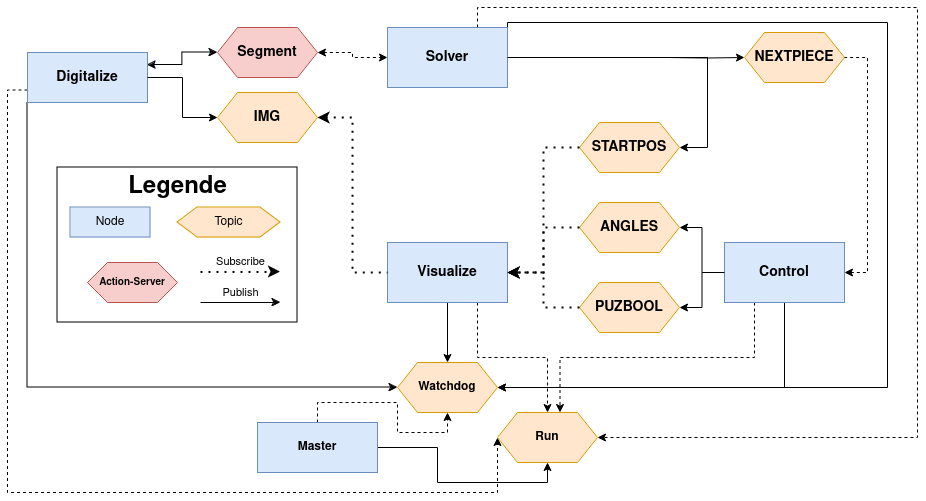
\includegraphics[width=1\textwidth]{Interfaces.png}
    \caption{Interfaces - In späteren Kapiteln genauer beschrieben}
\end{figure}

\newpage

\subsection{Zeitlicher Verlauf}
Der folgende Verlauf zeigt, wann im Projekt in etwa welche Aufgaben abgeschlossen wurden. Nachbesserungen, Anpassungen und Weiterentwicklungen sind weiterhin möglich.\\

\noindent\textbf{Wochen 1-4 (21.3.-18.4.)} 
\begin{itemize}
    \item Einteilung in Gruppen
    \item Einarbeitung in die jeweiligen Technologien
    \item Erstellung einer gemeinsamen Entwicklungsumgebung
    \item Aufnahmen der Puzzleteile anfertigen
    \item Einfache Roboterbewegung berechnen
\end{itemize}

\noindent\textbf{Woche 5 (18.4.-25.4.)} 
\begin{itemize}
    \item Entzerren der Aufnahmen
    \item Extraktion der Puzzleteilkanten
\end{itemize}

\noindent\textbf{Wochen 6-7 (25.4.-9.5.)} 
\begin{itemize}
    \item Visualisierung des Robotermodells
    \item Kantenvergleich als Wahrscheinlichkeitsmaß
    \item Erster Ansatz für Solveralgorithmus
    \item Segmentierung des Puzzleteils
    \item Berechnung Inverse Kinematik
\end{itemize}

\noindent\textbf{Wochen 8-9 (9.5.-23.5.)} 
\begin{itemize}
    \item Ground Truth Mock zum dynamischen Testen der Solving Algorithmen
    \item Postprocessing: Ausgaben der Solver Gruppe
    \item Interpolation Roboterbewegung 
\end{itemize}

\noindent\textbf{Wochen 10-11 (23.5.-6.6.)} 
\begin{itemize}
    \item optimierter Solveralgorithmus ”Best First + Global Best”
    \item Simulated Annealing
    \item Farbmatching der Puzzleteilkanten
    \item Grundsätzliche Visualisierung dreidimensionales Puzzleteil
    \item XOR Matcher der Puzzleteilkanten
    \item Entwicklung verschiedener Schnittstellen / ROS Nodes und Nachrichten
\end{itemize}

\noindent\textbf{Wochen 12-14 (6.6.-20.6.)} 
\begin{itemize}
   \item \textbf{Teilintegrationstests:} \\Zusammenfügen von verschiedenen Nodes und Test derer im Verbund \\ \underline{Szenarien:}
\begin{itemize}
\item Control\textless-\textgreater  Visualize: Bewegungsanimation Roboter
\item Digitalize\textless-\textgreater  Solve: Visualisierung Puzzle
\item Digitalize\textless-\textgreater  Solve: Lösen des Puzzles
\end{itemize}
\item Erstellung einer Master Node, die die einzelnen Komponenten zentral ansteuert
\end{itemize}

\noindent\textbf{Wochen 15-17 (20.6.-.4.7.)} 
\begin{itemize}
\item Integration aller ROS Nodes in ein Gesamtprodukt
\item Bugfixes
\item Dokumentieren des Projekts
\end{itemize}